\documentclass[tikz,border=4pt]{standalone}
\usepackage{fontspec}
\setsansfont{Latin Modern Sans}
\usepackage[none]{hyphenat}
\usetikzlibrary{positioning,arrows.meta,fit,backgrounds}
\begin{document}
\sffamily\footnotesize
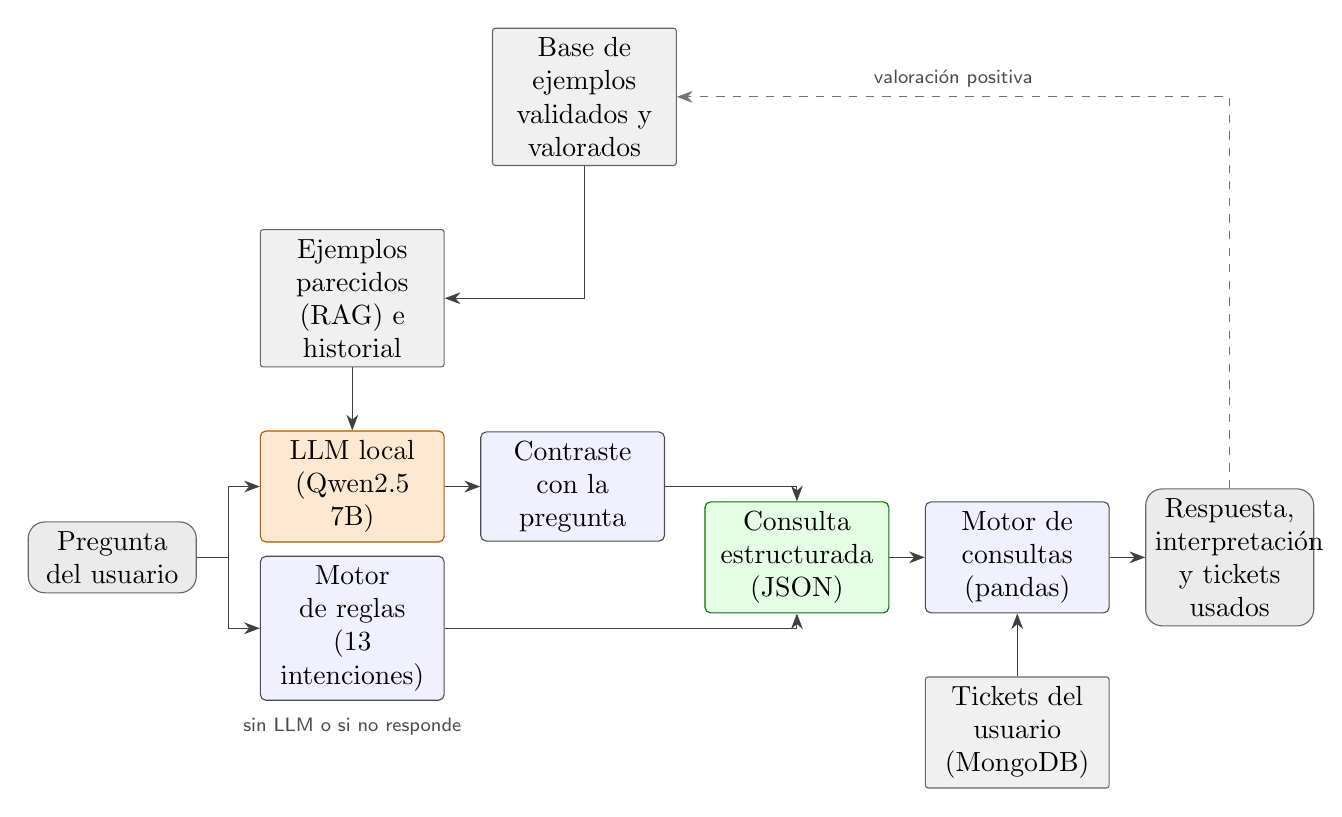
\begin{tikzpicture}[
  node distance=4mm and 4.5mm,
  paso/.style={draw=black!70, rounded corners=2pt, fill=blue!6, align=center, minimum height=11mm, text width=21mm},
  llm/.style={paso, fill=orange!18, draw=orange!70!black},
  datos/.style={draw=black!60, fill=black!6, align=center, text width=21mm, minimum height=9mm, rounded corners=1pt},
  fin/.style={draw=black!60, rounded corners=6pt, fill=black!8, align=center, text width=19mm, minimum height=9mm},
  flecha/.style={-{Stealth[length=2mm]}, black!75},
  discont/.style={-{Stealth[length=2mm]}, black!55, dashed},
  etiqueta/.style={font=\sffamily\scriptsize, black!70}]
\node[fin] (pregunta) {Pregunta del usuario};
\node[llm, right=8mm of pregunta, yshift=9mm] (llm) {LLM local\\(Qwen2.5 7B)};
\node[paso, right=8mm of pregunta, yshift=-9mm] (reglas) {Motor de reglas\\(13 intenciones)};
\node[paso, right=of llm] (ajustes) {Contraste con la pregunta};
\node[paso, anchor=west, fill=green!10, draw=green!45!black] (consulta) at ([xshift=5mm]ajustes.east |- pregunta) {Consulta estructurada (JSON)};
\node[paso, right=of consulta] (motor) {Motor de consultas (pandas)};
\node[fin, right=of motor] (respuesta) {Respuesta, interpretación y tickets usados};
\node[datos, above=8mm of llm] (rag) {Ejemplos parecidos (RAG) e historial};
\node[datos, below=8mm of motor] (tickets) {Tickets del usuario (MongoDB)};
\node[datos, above=8mm of rag.north east, anchor=south west, xshift=6mm] (base) {Base de ejemplos validados y valorados};
\draw[flecha] (pregunta.east) -- ++(4mm,0) |- (llm.west);
\draw[flecha] (pregunta.east) -- ++(4mm,0) |- (reglas.west);
\draw[flecha] (llm) -- (ajustes);
\draw[flecha] (ajustes.east) -| (consulta.north);
\draw[flecha] (reglas.east) -| (consulta.south);
\draw[flecha] (consulta) -- (motor);
\draw[flecha] (motor) -- (respuesta);
\draw[flecha] (tickets) -- (motor);
\draw[flecha] (rag) -- (llm);
\draw[flecha] (base.south) |- (rag.east);
\draw[discont] (respuesta.north) |- node[pos=0.75, above, etiqueta]{valoración positiva} (base.east);
\node[etiqueta, below=1mm of reglas] {sin LLM o si no responde};
\end{tikzpicture}
\end{document}
